% Options for packages loaded elsewhere
\PassOptionsToPackage{unicode}{hyperref}
\PassOptionsToPackage{hyphens}{url}
\documentclass[
  11pt,
]{scrartcl}
\usepackage{xcolor}
\usepackage[margin=1in]{geometry}
\usepackage{amsmath,amssymb}
\setcounter{secnumdepth}{-\maxdimen} % remove section numbering
\usepackage{iftex}
\ifPDFTeX
  \usepackage[T1]{fontenc}
  \usepackage[utf8]{inputenc}
  \usepackage{textcomp} % provide euro and other symbols
\else % if luatex or xetex
  \usepackage{unicode-math} % this also loads fontspec
  \defaultfontfeatures{Scale=MatchLowercase}
  \defaultfontfeatures[\rmfamily]{Ligatures=TeX,Scale=1}
\fi
\usepackage{lmodern}
\ifPDFTeX\else
  % xetex/luatex font selection
\fi
% Use upquote if available, for straight quotes in verbatim environments
\IfFileExists{upquote.sty}{\usepackage{upquote}}{}
\IfFileExists{microtype.sty}{% use microtype if available
  \usepackage[]{microtype}
  \UseMicrotypeSet[protrusion]{basicmath} % disable protrusion for tt fonts
}{}
\makeatletter
\@ifundefined{KOMAClassName}{% if non-KOMA class
  \IfFileExists{parskip.sty}{%
    \usepackage{parskip}
  }{% else
    \setlength{\parindent}{0pt}
    \setlength{\parskip}{6pt plus 2pt minus 1pt}}
}{% if KOMA class
  \KOMAoptions{parskip=half}}
\makeatother
\usepackage{longtable,booktabs,array}
\usepackage{calc} % for calculating minipage widths
% Correct order of tables after \paragraph or \subparagraph
\usepackage{etoolbox}
\makeatletter
\patchcmd\longtable{\par}{\if@noskipsec\mbox{}\fi\par}{}{}
\makeatother
% Allow footnotes in longtable head/foot
\IfFileExists{footnotehyper.sty}{\usepackage{footnotehyper}}{\usepackage{footnote}}
\makesavenoteenv{longtable}
\usepackage{graphicx}
\makeatletter
\newsavebox\pandoc@box
\newcommand*\pandocbounded[1]{% scales image to fit in text height/width
  \sbox\pandoc@box{#1}%
  \Gscale@div\@tempa{\textheight}{\dimexpr\ht\pandoc@box+\dp\pandoc@box\relax}%
  \Gscale@div\@tempb{\linewidth}{\wd\pandoc@box}%
  \ifdim\@tempb\p@<\@tempa\p@\let\@tempa\@tempb\fi% select the smaller of both
  \ifdim\@tempa\p@<\p@\scalebox{\@tempa}{\usebox\pandoc@box}%
  \else\usebox{\pandoc@box}%
  \fi%
}
% Set default figure placement to htbp
\def\fps@figure{htbp}
\makeatother
\setlength{\emergencystretch}{3em} % prevent overfull lines
\providecommand{\tightlist}{%
  \setlength{\itemsep}{0pt}\setlength{\parskip}{0pt}}
\usepackage{booktabs}
\usepackage{float}
\usepackage{caption}
\usepackage{setspace}
\usepackage{bookmark}
\IfFileExists{xurl.sty}{\usepackage{xurl}}{} % add URL line breaks if available
\urlstyle{same}
\hypersetup{
  pdftitle={Is Cholesterol Overrated? Examining Its Independent Effect on Heart Disease Risk},
  pdfauthor={Logan Calder, Chase Mayer, Anirudh Ramesh},
  hidelinks,
  pdfcreator={LaTeX via pandoc}}

\title{Is Cholesterol Overrated? Examining Its Independent Effect on
Heart Disease Risk}
\author{Logan Calder, Chase Mayer, Anirudh Ramesh}
\date{2026-04-14}

\begin{document}
\maketitle

\subsection{Introduction}\label{introduction}

\subsection{Data}\label{data}

\subsection{Data Visualization}\label{data-visualization}

\begin{figure}
\centering
\pandocbounded{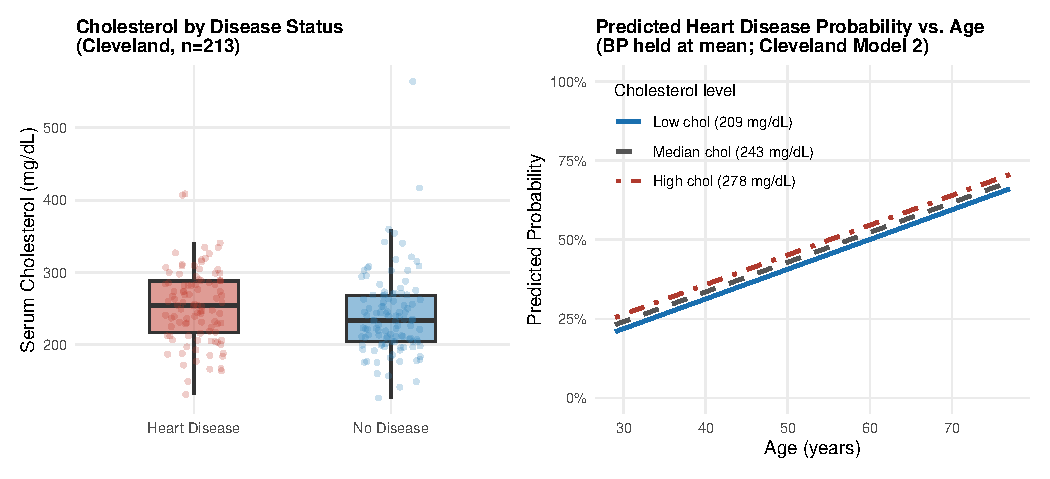
\includegraphics[keepaspectratio]{203_Rmd_Final_files/figure-latex/main-plot-1.pdf}}
\caption{Left: Right:}
\end{figure}

\subsection{Model Specification}\label{model-specification}

\subsection{Model Assumptions}\label{model-assumptions}

\subsection{Results and
Interpretation}\label{results-and-interpretation}

\begin{table}[H] \centering 
  \caption{Serum Cholesterol and Heart Disease Presence} 
  \label{} 
\footnotesize 
\begin{tabular}{@{\extracolsep{5pt}}lcccc} 
\\[-1.8ex]\hline 
\hline \\[-1.8ex] 
 & \multicolumn{4}{c}{\textit{Dependent variable:}} \\ 
\cline{2-5} 
\\[-1.8ex] & \multicolumn{4}{c}{Heart Disease (1 = present, 0 = absent)} \\ 
 & \multicolumn{2}{c}{Cleveland Only} & \multicolumn{2}{c}{All Four Sites} \\ 
\\[-1.8ex] & (1) & (2) & (3) & (4)\\ 
\hline \\[-1.8ex] 
 Serum Cholesterol (mg/dL) & 0.001 & 0.001 & 0.001$^{***}$ & 0.001$^{**}$ \\ 
  & (0.001) & (0.001) & (0.0003) & (0.0003) \\ 
  Age (years) &  & 0.009$^{**}$ &  & 0.013$^{***}$ \\ 
  &  & (0.004) &  & (0.002) \\ 
  Resting Blood Pressure (mmHg) &  & 0.004$^{*}$ &  & 0.003$^{***}$ \\ 
  &  & (0.002) &  & (0.001) \\ 
  Constant & 0.191 & $-$0.671$^{**}$ & 0.224$^{***}$ & $-$0.779$^{***}$ \\ 
  & (0.188) & (0.293) & (0.082) & (0.166) \\ 
 \hline \\[-1.8ex] 
Observations & 213 & 213 & 675 & 675 \\ 
R$^{2}$ & 0.016 & 0.068 & 0.014 & 0.097 \\ 
Adjusted R$^{2}$ & 0.011 & 0.055 & 0.012 & 0.093 \\ 
Residual Std. Error & 0.498 (df = 211) & 0.487 (df = 209) & 0.497 (df = 673) & 0.476 (df = 671) \\ 
F Statistic & 3.415$^{*}$ (df = 1; 211) & 5.116$^{***}$ (df = 3; 209) & 9.473$^{***}$ (df = 1; 673) & 23.928$^{***}$ (df = 3; 671) \\ 
\hline 
\hline \\[-1.8ex] 
\textit{Note:}  & \multicolumn{4}{l}{$^{*}$p$<$0.1; $^{**}$p$<$0.05; $^{***}$p$<$0.01} \\ 
 & \multicolumn{4}{l}{Robust (HC3) standard errors in parentheses.} \\ 
\end{tabular} 
\end{table}

\subsection{Conclusion}\label{conclusion}

\newpage

\subsection{Appendix}\label{appendix}

\textbf{Model Specifications Tried.}

\begin{longtable}[]{@{}
  >{\raggedright\arraybackslash}p{(\linewidth - 2\tabcolsep) * \real{0.5000}}
  >{\raggedright\arraybackslash}p{(\linewidth - 2\tabcolsep) * \real{0.5000}}@{}}
\toprule\noalign{}
\begin{minipage}[b]{\linewidth}\raggedright
Specification
\end{minipage} & \begin{minipage}[b]{\linewidth}\raggedright
What We Learned
\end{minipage} \\
\midrule\noalign{}
\endhead
\bottomrule\noalign{}
\endlastfoot
\texttt{heart\_disease\ \textasciitilde{}\ chol} (Cleveland) & Baseline;
chol coefficient positive but not significant (\(p \approx 0.26\)) \\
\texttt{heart\_disease\ \textasciitilde{}\ chol\ +\ age\ +\ trestbps}
(Cleveland) & Adding age drives \(R^2\) up; chol becomes smaller and
still insignificant \\
\texttt{heart\_disease\ \textasciitilde{}\ chol} (All four sites) &
Larger \(n\) makes chol significant, but effect size unchanged \\
\texttt{heart\_disease\ \textasciitilde{}\ chol\ +\ age\ +\ trestbps}
(All four sites) & Both age and BP now significant; chol marginally
significant \\
\texttt{heart\_disease\ \textasciitilde{}\ log(chol)\ +\ age\ +\ trestbps}
& Log transform did not improve residual pattern or interpretation;
dropped \\
\texttt{heart\_disease\ \textasciitilde{}\ chol\ +\ I(chol\^{}2)\ +\ age\ +\ trestbps}
& Squared term not significant; residuals showed no curvature;
dropped \\
\end{longtable}

\textbf{Residuals vs.~Fitted Values Plot.}

\begin{figure}
\centering
\pandocbounded{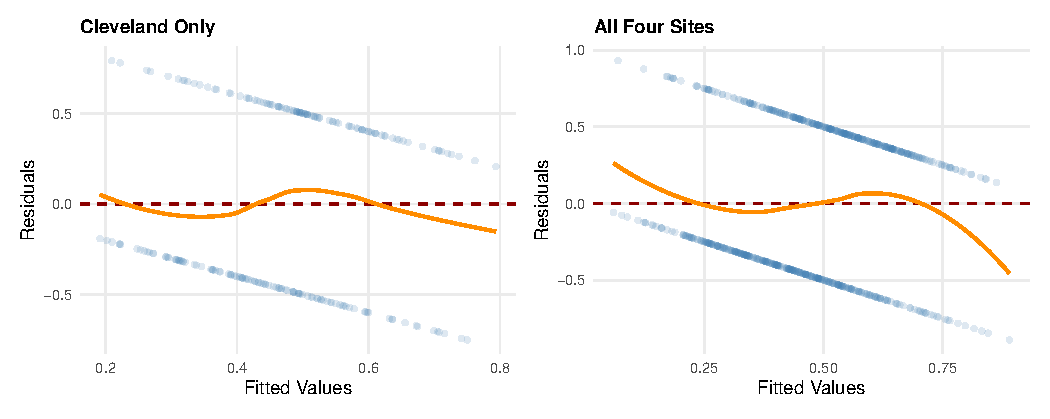
\includegraphics[keepaspectratio]{203_Rmd_Final_files/figure-latex/resid-plot-1.pdf}}
\caption{Residuals vs.~fitted values for Model 2 (cholesterol + age +
resting BP). Left: Right:}
\end{figure}

\end{document}
